\section{MTC device data upload procedure in LTE}
\label{sec:LTE-random-access}
We only concern about periodic MTC traffic whose work-flow is presented in a general way in Fig.\ref{fig:Time-driven M2M work flow}. It consists of user cases where low mobility or fixed devices periodically report collected data with small payload (less than $200$ bytes according to~\cite{HealthInformatics}) 
to remote servers. Consider a situation where a device  stays in RRC\_Idle state before starting its data reporting procedure.
\begin{figure}[!t]
	\centering
	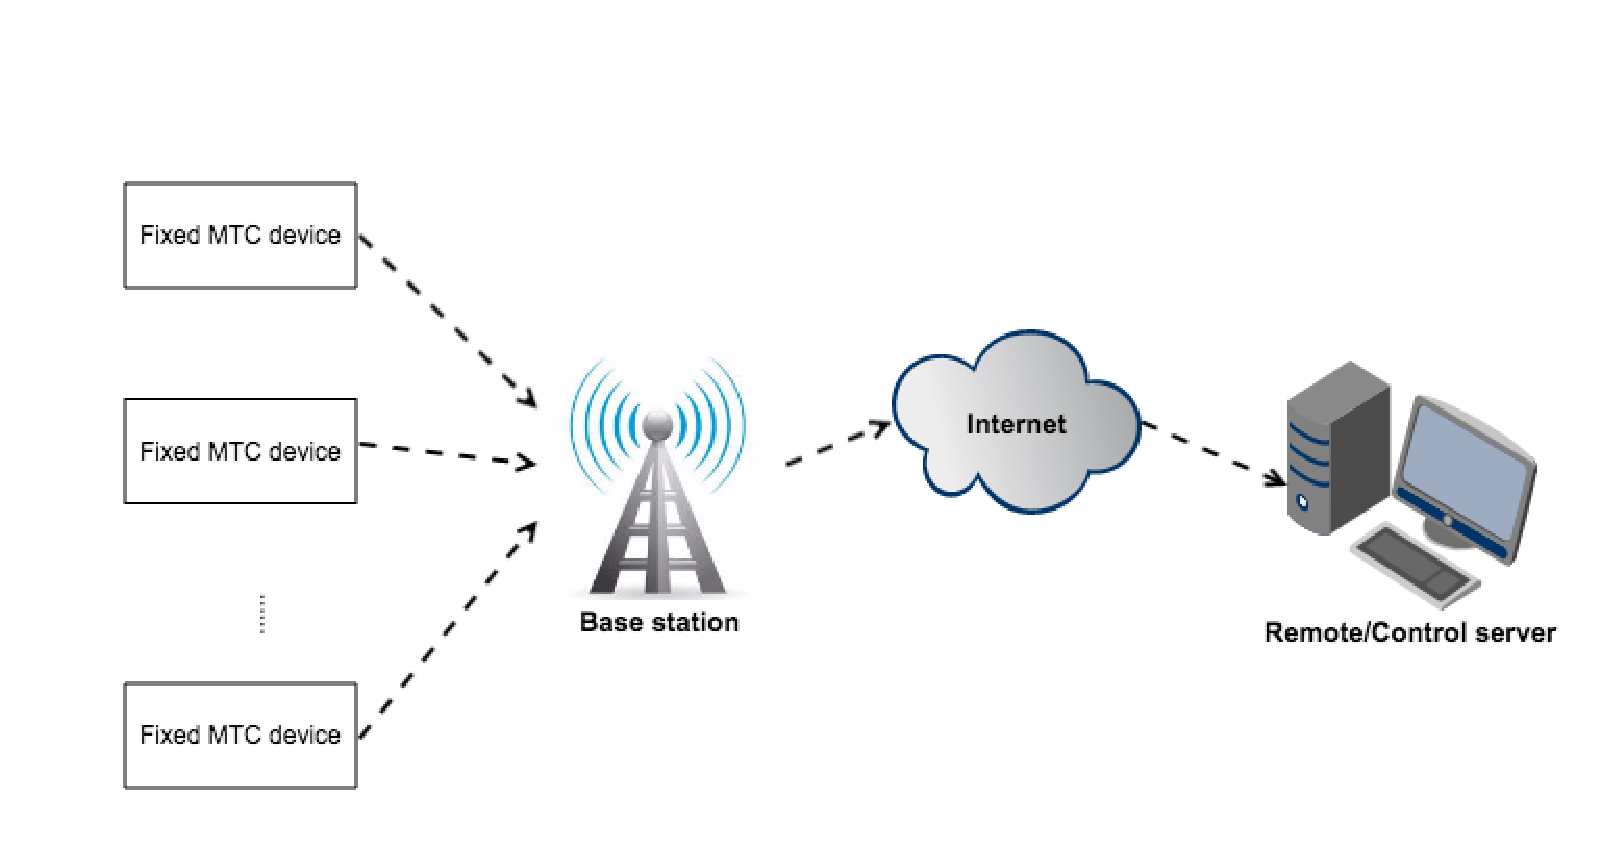
\includegraphics[width=\linewidth]{Chapter6/Figures/Time-driven-work-flow.eps}
	\caption{Periodic M2M application  work flow}
	\label{fig:Time-driven M2M work flow}
\end{figure}
Deployed in current LTE network, to finish data transmission, a device should repetitively go through three procedures: contention-based random access procedure for establishment of RRC connection, data transmission and release of established RRC connection. Note that term device and UE are used interchangeably in the rest of this chapter.
\subsection{Random access procedure}
\begin{figure*}[!t]
	\centering
	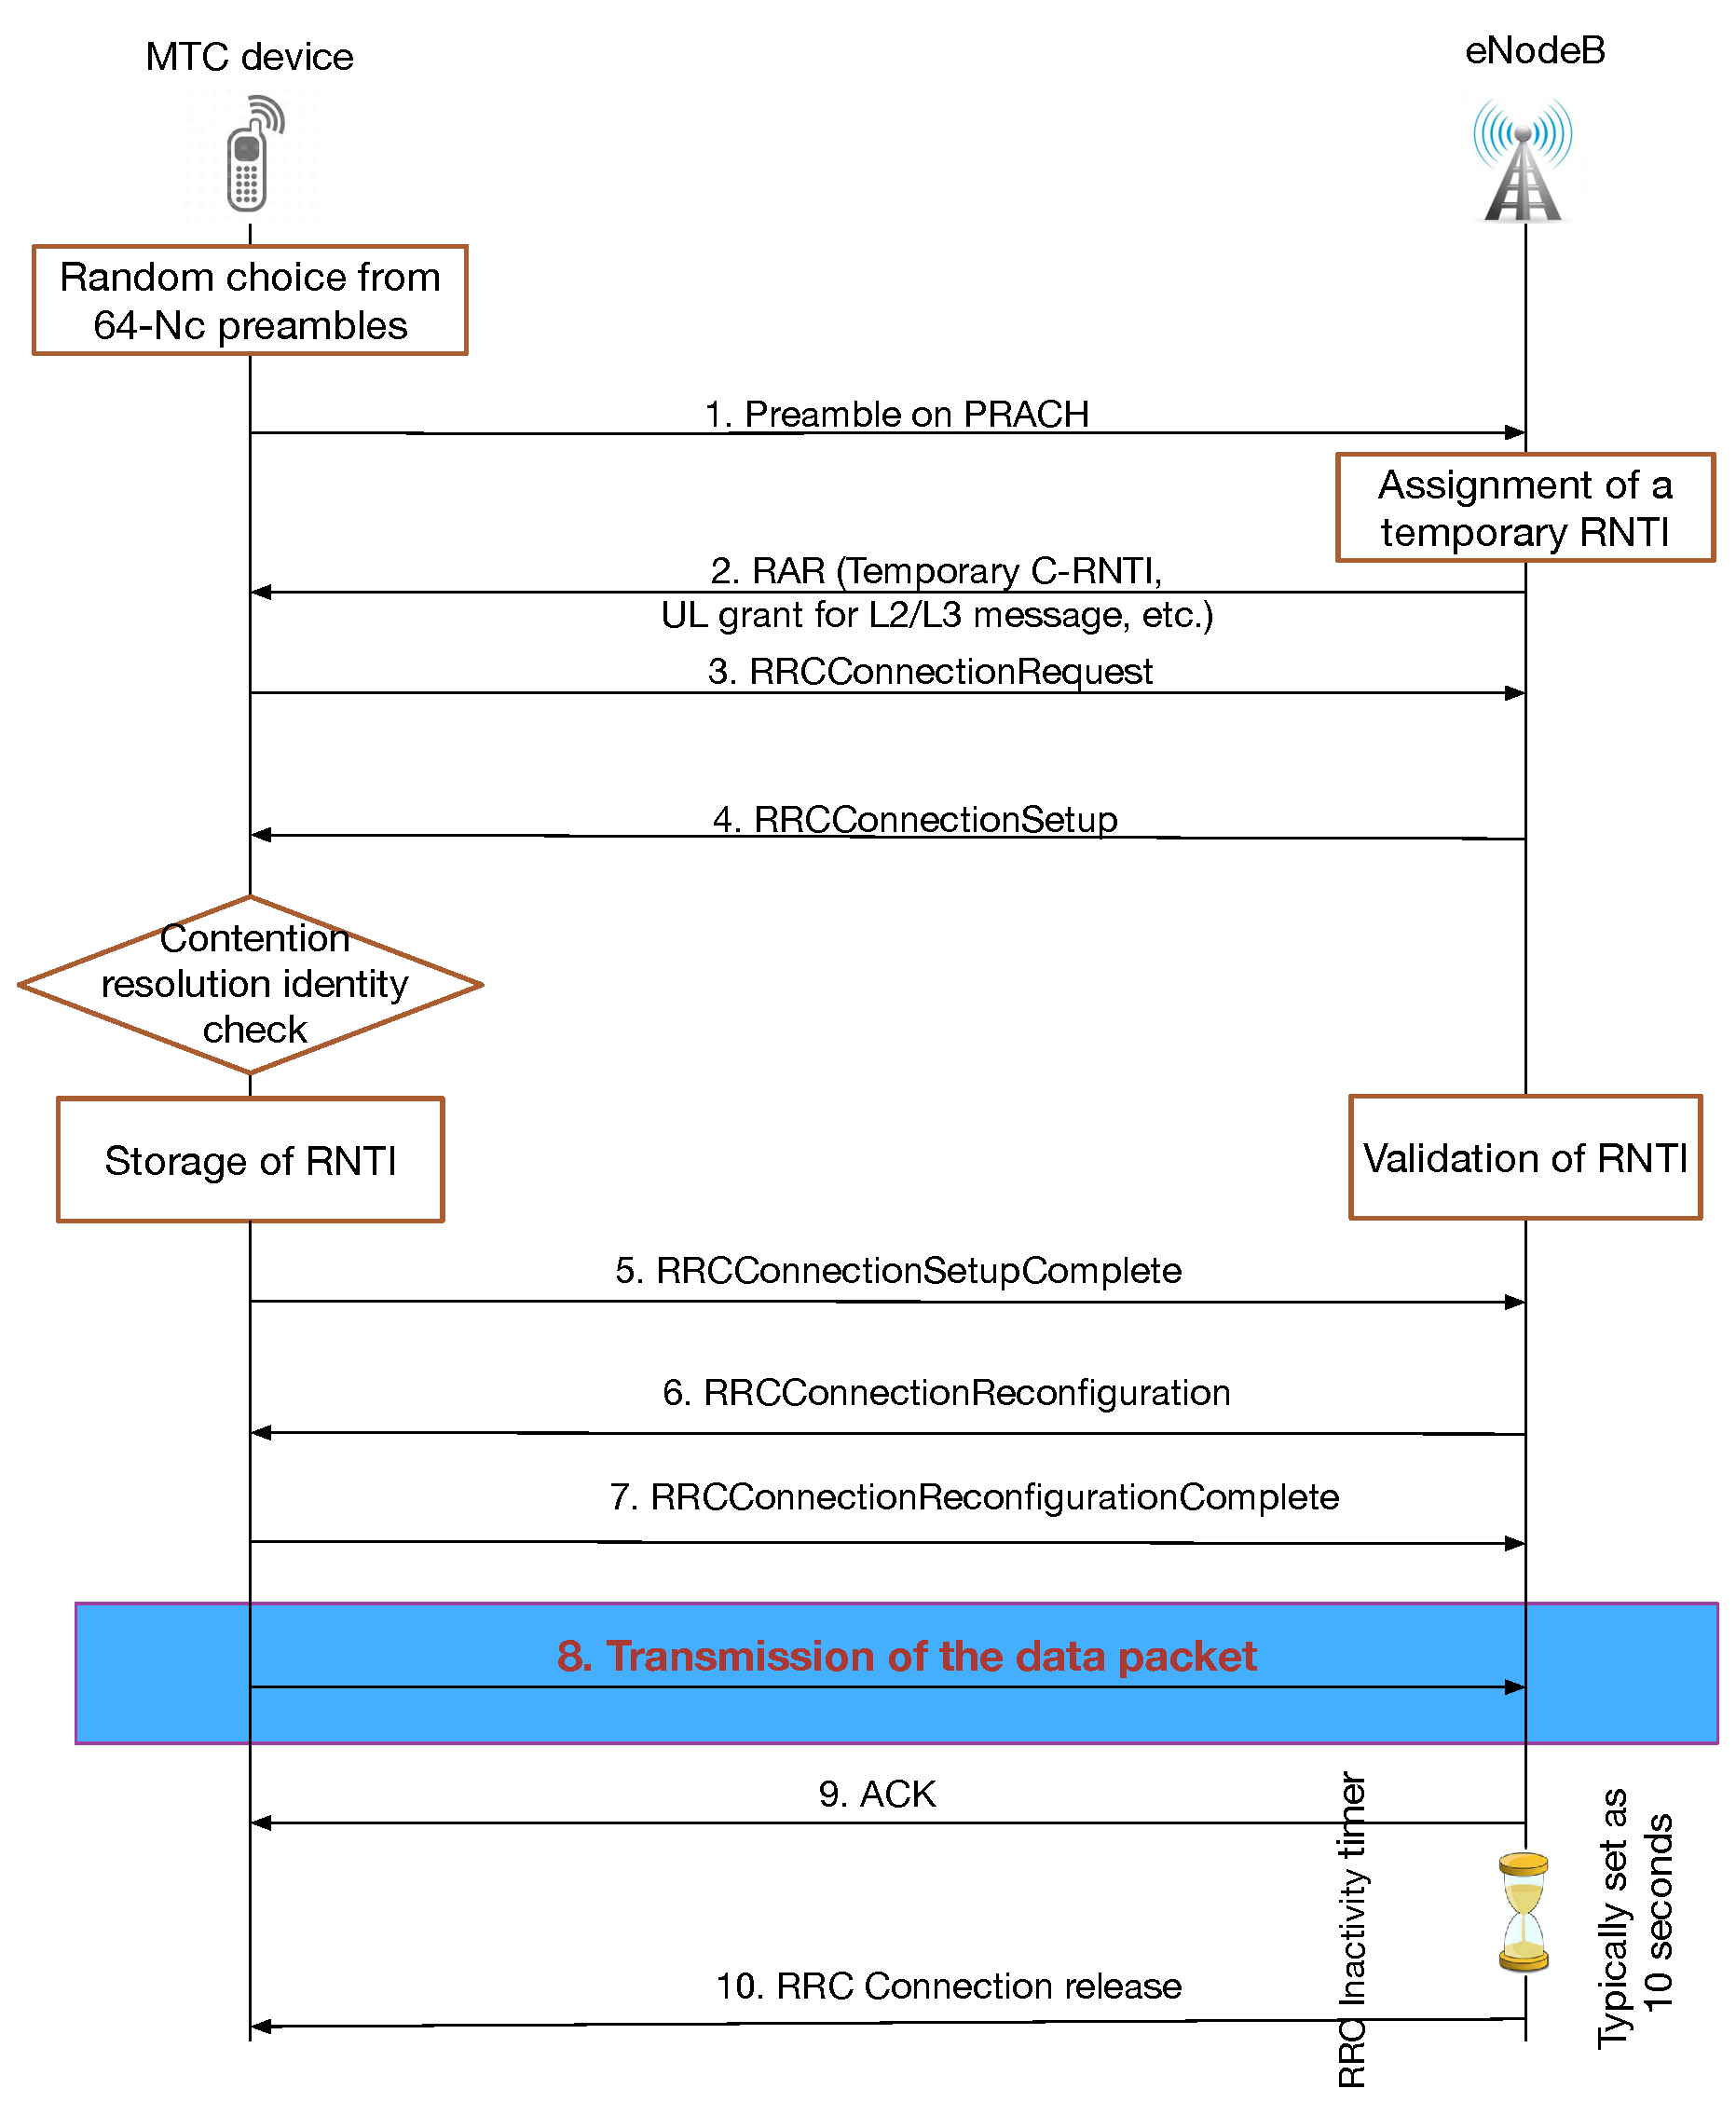
\includegraphics[width=\linewidth]{Chapter6/Figures/lte-ra.eps}
	\caption{Random access and data upload procedure in LTE networks}
	\label{fig:lte-ra}
\end{figure*}
As illustrated in Fig.~\ref{fig:lte-ra}, the random access procedure mainly consists of four steps presented as following. 
% 拉格朗日对这部分的建议是,到第四步再写 collision的情况
\begin{description}[font=\normalfont]
	\item[Step 1: Preamble transmission]\hfil \\
	In this step, the UE randomly selects one from the $64-N_c$ random access preambles and transmits the selected preamble at the next physical random access channel (PRACH) opportunity, where $N_c$ is the number of preambles reserved for non-contention based random access. After the preamble transmission, the UE shall monitor the PDCCH channel and try to decode a Random Access Response identified by the RA-RNTI from the eNB. %Note that the method to construct RA-RNTI is the same for UEs and eNB:
	% 每一步的写作思路是,先描述entity (UE, eNB) 内部如果运作,最后向对方发送什么内容,以及发送后的行为
	% 参考内容:
	% weblink : http://nitintayal-lte-tutorials.blogspot.fr/2013/09/random-access-procedure-rach.html
	% The mail answered by Xavier
	% Book: LTE-The UMTS Long Term evolution, from theory to practice	
	\item[Step 2: Random Access Response (RAR) ]\hfill \\
	%	After receiving RACH request in step1, The eNB PHY (Physical layer) calculates the timing advance which is transmitted to the UE as part of response message. %http://nitintayal-lte-tutorials.blogspot.fr/2013/09/random-access-procedure-rach.html
	The RAR message generated by the eNB is decoded with UE-generated RA-RNTI and contains the identity of the detected preamble, uplink channel synchronization information, an initial uplink resource grant for the transmission of the step 3 message, an assignment of a temporary Cell Radio Network Temporary Identifier (C-RNTI) along with other information. 
	\item[Step 3: L2/L3 message] \hfill \\
	%MSG3 (RRC Connection Reqeust)
	In this step, the UE sends the messages related to RRC connection request for random access procedure and makes use of Hybrid Automatic Repeat reQuest (HARQ). It is addressed to the temporary C-RNTI allocated in RAR at step 2 and carries the contention resolution identity. The contention resolution identity is a locally unique identity of the UE, which is generally built with the S-TMSI. After the transmission of step 3, the UE wait for the contention resolution message.
	\item[Step 4: Contention Resolution Reception] \hfill \\
	The contention resolution message from the eNB is addressed to the temporary C-RNTI and contains contention resolution identity received in L2/L3 message. This is an echo mechanism: if the UE detects its own identity, it knows that its random access request is accepted by eNB. If not, UE can infer that collision happens in previous step. A collision is occurred if more than one UEs select and send the same preamble to eNB in step 1. Each of them receives the same RAR in step 2 and thus uses the same same temporary C-RNTI in step 3. Either none of devices receives contention solution message and all colliding UEs restart from step 1, or just one of them receives echo and finishes the random access procedure.
\end{description}


\subsection{Transmission of data packet}
Since upload of MTC device data consists of a UE triggered service request procedure, L2/L3 message in previous is actually a RRCConnectionRequest and Contention resolution message is RRCConnectionSetup. Subsequently the UE sends service request in message RRCConnectionSetupComplete. After an exchange of RRCConnectionReconfiguration, UE establishes a RRCConnection network and starts the data transmission.
% http://lteuniversity.com/get_trained/expert_opinion1/b/lauroortigoza/archive/2013/12/18/rrc-connection-release.aspx
% 参考这一部分
\subsection{RRC Connection Release}
After transmission of data packet, UE goes back to RRC\_Idle state after the expiration of RRC inactivity timer, eNB deletes complete UE context and releases the established RRC connection with UE. Thus, UE has to pass through above steps before getting a RNTI for the next reporting.

With above description, traditional RACH access method poses some challenges when handling MTC in particular periodic MTC traffic. First massive device requests may lead to access network congestion. Second the control signaling overhead for small payload (e.g. $100$ bytes) is expensive, for example acquiring radio access network resources requires at least four messages exchanged between devices and network. Third short transaction for small payload causes inefficient resource utilization. Taking the consumption of RNTI as an example: assuming a MTC device needs to send $100$ bytes to remote server,  with a robust modulation scheme, the transmission is usually finished in $100$ ms, MTC device does not need to hold allocated RNTI until next reporting. However, the eNB has no way to determine whether device has data to transmit and takes back allocated RNTI after the expiration of related timer. 
%In addition, if periodic M2M application recoveries from a power outage, all managed MTC devices simultaneously try to connect eNB, which leads to a high collision level in radio access network. 
%Therefore, current RACH leads to waste of system resource and high overhead for each transmission if directly applied for MTC.
% 修改这部分标题,Xavier的意思是 这是直接在reseau de transport中提供的一种service 所以
